\subsection{Test vehicle description}

% Why making a testchip
It is difficult to realize good measurements on an integrated circuit.
The chip is enclosed in a package, and without physical access it is impossible to measure electrical properties.
Even with physical access, placing micro-probes to contact metal connections can disturb sensitive parts of the device.
To overcome these issues, it is interesting to develop custom structures that perform the measurements directly on the chip and output the data using standard \gls{io}.
For that matter, a custom test vehicle has been designed and manufactured.

% What is in the testchip
The testchip reuses most blocks from the Everest product described previously in \ref{sec:study-real-product}.
%TODO: What is monitored
In addition, custom functions were integrated to allow the measurement and monitoring of internal parameters.
A communication system was setup to output measurement data using a few pins.

% Why monitoring a primary supply
The studied function is the primary supply of a complex automotive \gls{asic}.
This supply plays a critical role in the functionning of the entire product.
It is connected to the battery of the vehicle, and is the first block of the product to start.
It wakes up and powers all other functions inside the integrated circuit.

% Global architecture
The global architecture of the testchip (Fig. \ref{architecture_testchip}) is comprised of a duplicated supply function.
The same supply block is instanciated twice on silicon.
One of them is the function under test, which is exposed to \gls{ESD} stresses and is monitored for failures.
The second one is responsible for powering the monitoring functions.
Both blocks are isolated from one another as much as possible.
The monitoring's supply is protected against disturbances to ensure good measurements.

\begin{figure}[h]
  \centering
  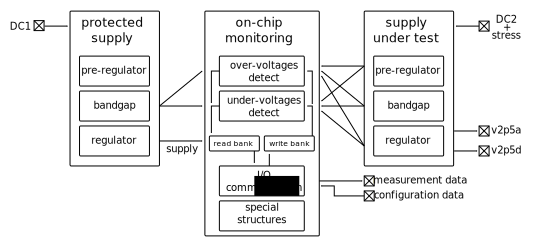
\includegraphics{src/3/figures/architecture_testchip.pdf}
  \caption{Global architecture of the test vehicle}
  \label{architecture_testchip}
\end{figure}

% What is in the monitoring system
The monitoring system is comprised of several functions.
Overvoltage and undervoltage detectors monitor voltage on nets in the supply under test.
The communication function performs a parallel to serial conversion, in order to read and write a large amount of bits using just a few pins.
Special structures for specific monitoring functions is also implemented.
Details about the monitored and monitoring functions are given in the next sub-sections.

\subsection{Supply function under monitoring}

% Main task
The main function of the supply block is mostly to down-convert a battery voltage to a 2.5V regulated supply.
Several blocks are involved for processing the battery supply.
The overall architecture is given in fig. \ref{fig:monitored_function}).

% First block
First, a pre-regulator clamps the battery voltage that can reach 40V down to a 9V.
This is done to protect more sensitive circuits connected downstream.
This output has low current capability and is used for low-power functions.
A second output provides a 12V clamped output with a large current capability.

% Second block
A bandgap reference is connected downstream.
It is powered by the 9V supply.
Once properly started after a certain delay, the bandgap generates a 1.23 V voltage reference.
This reference is stable accross a wide range of temperature, process variation and process mismatchs.
The bandgap also outputs a 10uA current reference, and a flag \textit{bgok} to signal it is ready for operation.

\begin{figure}[!htbp]
  \centering
  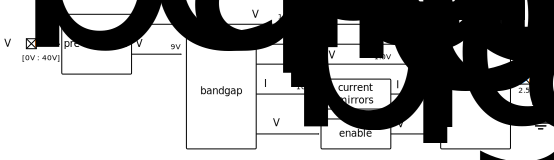
\includegraphics[width=0.9\textwidth]{src/3/figures/monitored_function.pdf}
  \caption{Architecture of the supply under test}
  \label{fig:monitored_function}
\end{figure}

% Third major block
Finally, the \gls{ldo} regulator generates a stable 2.5V supply voltage, able to deliver and sustain up to 20mA.
In the original product, this output is used further in the system to power digital gates.

% Detail nets connections
The regulator relies on multiple signals generated in the upstream blocks for operation.
The most critical nets are the 1.0V reference from the bandgap, and the ramp-up signal.
Circuit analysis show that both nets can directly affect the output voltage.
A variation on the reference voltage is immediately copied on the output.
The ramp-up signal controls the soft-start of the regulator, that can directly change the output value.
Other nets provide bias to the regulator, and their impact on the output is more limited.

% Talk about external devices
The regulator is connected externally to a 100nF decoupling capacitor to absorb peak currents and achieve stability.

% What are the minor blocks doing
The \textit{current mirrors} provide copied current values from the bandgap, while offering much larger output impedance.
The \textit{enable} block mostly checks and waits for the bandgap to be properly started.
It then triggers a startup ramp-up sequence on the regulator.

\subsection{Voltage monitoring}

% What are the OV/UV detectors made of
Overvoltage and undervoltage detectors are implemented as latched comparators.
They record if a monitored net crosses a threshold.
The latch behavior stores the value until it can be read.
The architecture of a detector is given Fig. \ref{fig:architecture-ov}.
The same architecture is used for the overvoltage and the undervoltage.
Monitored and reference inputs are just inversed on the undervoltage detector.

\begin{figure}[!htbp]
  \centering
  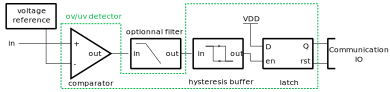
\includegraphics[width=0.9\textwidth]{src/3/figures/architecture_OV.pdf}
  \caption{Architecture of the overvoltage detector}
  \label{fig:architecture-ov}
\end{figure}

% What is the purpose of filter
%TODO
Optional filter, with hysteresis threshold, to evaluate duration of violation

% Origin of reference voltages
The reference voltages for these comparators come from the protected supply.
The comparators monitor several key voltages inside the supply under test.
The output of these latched comparators form a register bank of 35 bits.

%TODO: Detail

\subsection{Communication system}

% What does the comm IO
The monitoring system also provides a bidirectionnal communication system.
It is designed to read with a single pin the values from the comparator register bank.
It also supports writing to a second register bank, that is used in the monitoring system for configuration.

%TODO: Detail

\subsection{On-chip near-field current sensors}

To be done
%TODO: Refer to PhD Alain
%TODO: Use document These/07
